\documentclass[a4paper,12pt]{article}
\usepackage[francais]{babel}
\usepackage{graphicx}
\usepackage{geometry}

\geometry{ hmargin=2.5cm, vmargin=2.5cm }
\title{Programmation I : DM2 - Chameaux} 
\author{Anne-Laure MOULY et Vincent DELAITRE}

\begin{document}
\maketitle
\section{Strategies}
\subsection{Attaque}
Notre chameau ne cherche, en g\'en\'eral, pas les probl\`emes. Disons qu'il ne va pas chercher un adversaire \`a l'autre bout de la carte pour lui faire des mis\`eres (sauf s'il n'y a plus de $\lambda$-termes sur la carte, auquel cas il peut devenir agressif). Cependant, il vaut mieux pour les autres ne pas se balader trop pr\`es quand m\^eme.\\
En effet la partie Attaque de notre chameau s'active lors qu'un adversaire est situ\'ee \`a moins de 3 cases (\`a vol d'oiseau). Notre chameau essaye alors d'effectuer les actions suivantes dans l'ordre:
\begin{enumerate}
\item Si on peut pousser quelqu'un au contact dans un omega, on ne s'en prive pas (dans les illustrations ci-dessous, notre chameau est le gentil donc le clair, les m\'echants sont en sombre par d\'efinition du c\^ot\'e obscur de la force):
\begin{center}
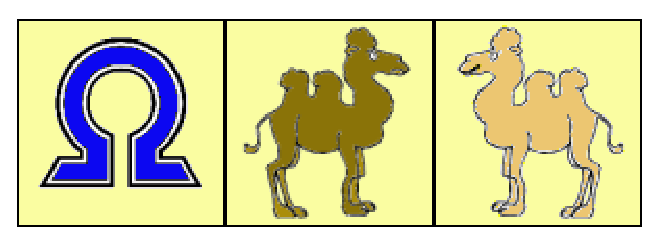
\includegraphics[scale=0.3]{./graph001.eps}
\end{center}
\item Si on peut pousser dans un omega en moins d'un certain nombre de coups (r\'egl\'e \`a 4 actuellement), on tente notre chance:
\begin{center}
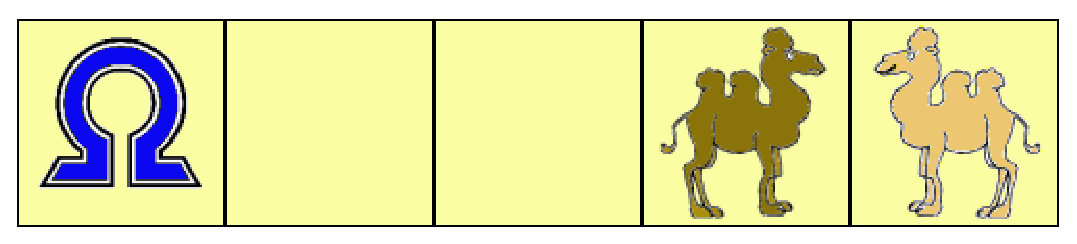
\includegraphics[scale=0.3]{./graph002.eps}
\end{center}
\item Si on peut pousser quelqu'un qui n'est pas au contact mais qui va peut \^etre y aller, on essaye:
\begin{center}
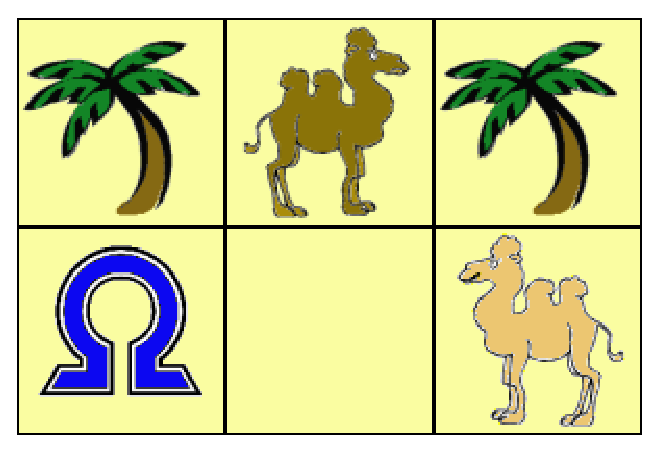
\includegraphics[scale=0.3]{./graph003.eps}
\end{center}
\item Si on pourra pousser quelqu'un au prochain tour, on y va:
\begin{center}
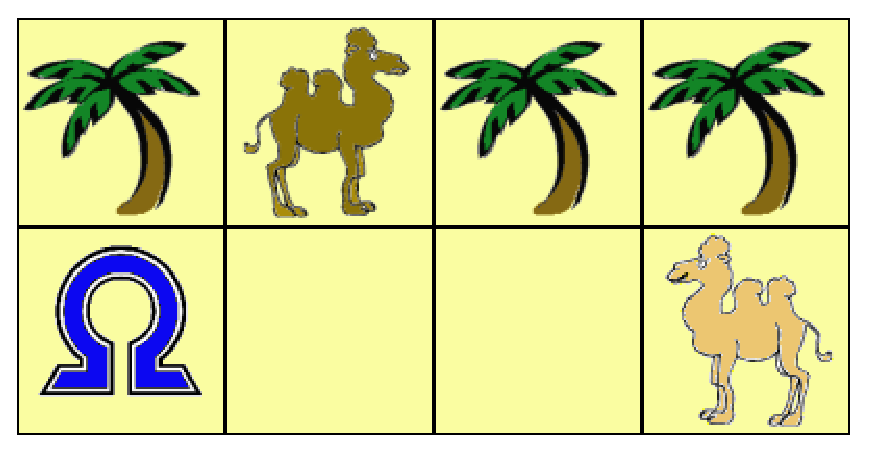
\includegraphics[scale=0.3]{./graph004.eps}
\end{center}
\item Si Sauve pr\'econise de ramasser des $\lambda$-termes, on regarde si ca vaut le coup: si oui, on les rammasse, si non, ceux qui ont programm\'e Sauve sont d\'ebiles.
\item Si un m\'echant au contact avec nous est sur une base: on le pousse (sauf s'il y a un palmier derri\`ere lui: il ne bougerait pas), parce que les bases, c'est pour nous.
\item Si le gain est suffisant, on peut pousser un m\'echant pour r\'ecup\'erer ses $\lambda$-termes (sauf s'il y a un palmier derri\`ere lui: on ne pourrait pas rammasser ce qu'il a perdu, \c ca serait balot). Pour calculer le gain potentiel, on proc\`ede de la mani\`ere suivante:
\begin{itemize}
\item Soit $C_{totale}$ la capacit\'e d'un chameau et $C_{libre}$ la place libre qu'il reste \`a notre chameau. Soit $T$ l'ensemble des $\lambda$-termes que porte le m\'echant. On note $|t|$ la taille d'un terme \'el\'ement de $T$.
\item Soit $Somme_{vol}$ la somme des tailles des $\lambda$-termes sur le m\'echant et que l'on peut ramasser: $Somme_{vol}=\displaystyle{\sum_{t\in T, |t|<C_{libre}}{|t|}}$. Un terme dont la taille est inconnue compte pour [taille moyenne]*[proba qu'on puisse le prendre] dans le total, soit $\displaystyle{[\frac{C_{totale}}{2}]*[\frac{C_{libre}}{C_{totale}}]=\frac{C_{libre}}{2}}$\\
Alors la taille moyenne du $\lambda$-terme que l'on va rammasser sera $vol=\displaystyle{\frac{Somme_{vol}}{card(T)}}$
\item On ajoute \`a $vol$ tous les $\lambda$-termes qui \'etaient d\'ej\`a par terre et que l'on peut ramasser pour avoir $Somme_{totale}$. $Somme_{totale}$ ne peut donc pas d\'epasser $C_{libre}$.
\item Malheureusement, on doit passer un tour \`a ramasser les $\lambda$-termes et le m\'echant va nous pousser: on va perdre un $\lambda$-terme de valeur moyenne:\\ $perte=\displaystyle{\frac{C_{totale}-C_{libre}+Somme_{totale}}{\textrm{nombre de termes total (ramass\'es+anciens)}}}$
\item Le gain moyen est alors: $gain=Somme_{totale}-perte$
\end{itemize}
\end{enumerate}
Toutes les actions \'enum\'er\'ees ci-dessus ne mettent pas notre chameau en danger, mais ne le sauve pas s'il est d\'ej\`a en danger (d'o\`u l'utilit\'e du module D\'efense). Pour choisir efficacement qu'elle action on ex\'ecute, on calcule une repr\'esentation des altentours dans un tableau 7*7, centr\'e sur notre chameau, dont je donne ci-dessous une repr\'esentation graphique:
\begin{center}
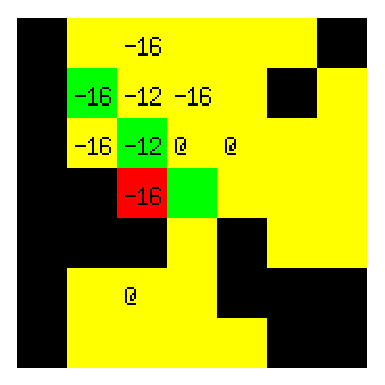
\includegraphics[scale=0.6]{./alentours.eps}
\end{center}
La l\'egende est la suivante:
\begin{itemize}
\item noir: case infranchissable
\item jaune: sable
\item rouge: case o\`u il vaut mieux ne pas aller car on se mettrait alors en danger de mort.
\item vert: case int\'eressante car permet de pousser un m\'echant dans un omega, soit parce qu'il est d\'ej\`a en danger, soit parce qu'il s'y exposera peut-\^etre au tour prochain (pour cela on calcule la probabilit\'e de d\'eplacement d'un m\'echant sur une case donn\'ee avec les poids suivants: le m\'echant reste sur place ou recule: poids 1, le m\'echant avance: poids 3, le m\'echant prend une autre direction: poids 2)
\item chiffre ou @: gain potentiel ou base
\end{itemize}
On choisit alors l'action \`a effectuer en fonction de la couleur de la case sur laquelle notre gentil chameau se trouve et les 4 voisines environnantes.
\subsection{R\'eponse \`a une question cruciale: combien miser?}
Au moins on sait que quand on n'attaque ni ne d\'efend, on mise 1. Apr\`es, pas de certitudes... Au niveau du signe de la mise pas trop de probl\`eme, suivant les situations, on sait si l'on veut agir avant ou apr\`es le m\'echant. Le probl\`eme est vraiment de savoir combien miser. On a donc d\'ecid\'e de faire une mise qui \'evolue suivant que l'on perd ou l'on gagne un duel. Chaque m\'echant se voit attribuer une mise optimale qui correspond \`a un certain pourcentage de l'eau r\'eserv\'ee au combat (=eau-(nombre maximum de tour que notre chameau joue avant d'\^etre \'eject\'e par le serveur)). Lorsque qu'on perd un duel: on multiplie cette mise optimale par un certain coefficient pour l'augmenter, idem lorsque l'on gagne pour la r\'eduire (pour \'economiser l'eau, si pr\'ecieuse dans un d\'esert). On se limite quand m\^eme \`a une mise maximum pour pas mourrir de soif qui est calcul\'e \`a partir de la fr\'equence des combats, de l'eau qu'il nous reste et du nombre de tours qu'il reste \`a jouer.\\
La question n'est cependant pas compl\`etement r\'esolue: combien miser pour pousser dans l'omega (ou ne pas \^etre pouss\'e, telle est la question)? Certains diront beaucoup... certes mais combien? Si on d\'efend \c ca doit bien tourner autour de 80\% de notre r\'eserve d'eau, mais si on attaque, sachant que l'autre va miser 80\%, est-on pr\^et \`a en faire autant? Cela reste une question ouverte. Pour l'instant, nous faisons l'autruche en refusant de voir le probl\`eme et on mise 10 fois la mise maximale calcul\'ee ci-dessus...
\section{Tests}
\subsection{G\'en\'erateur de carte}
Pour tester notre b\'eb\'e (chameau), nous avons fait un g\'en\'erateur de carte. Pour l'utiliser il faut d'abord cr\'eer un fichier .par (voir ci-dessous) puis lancer:\\
./mapgen $nom_du_fichier_par$\\
par exemple, avec un fichier test.par, on tape ./mapgen test et il g\'en\`ere test.lterm et test.map.\\
Le fichier .par comprend les champs suivant:\\
\begin{itemize}
\item LARGEUR: la largeur de la carte
\item HAUTEUR: la hauteur de la carte
\item CAPACITE\_MAX: la taille maximale des $\lambda$-termes
\item NB\_CHAMEAUX: le nombre maximum de joueurs
\item NB\_LTERMS: le nombre de $\lambda$-termes
\item NB\_BASES: le nombre de bases
\item FREQ\_OMEGA: la fr\'equence des omegas sur la carte
\item FREQ\_PALMIER: la fr\'equence des palmiers sur la carte
\item FREQ\_SABLE: la fr\'equence du sable sur la carte
\item MAGIC\_NUMBER: le nombre pour initialiser le g\'en\'erateur de nombres al\'eatoires
\end{itemize}
Avec tout \c ca on peut faire plein de choses, mais le g\'en\'erateur ne garantit pas que la carte n'a qu'une composante connexe: il possible qu'un chameau ne puisse pas atteindre une base ou sauver un $\lambda$-terme, dur la vie.
\subsection{R\'esultats exp\'erimentaux en solo}
\scriptsize{
\begin{center}
\begin{tabular}{|c|c|c|c|c|c|}
\hline
\multicolumn{2}{|c|}{IA\_sauve\_chemin.ml} & IA\_sauve\_ramasse.ml & \multicolumn{2}{|c|}{IA\_sauve\_livre.ml} &\\
\hline
trouve\_chemin & ameliore\_chemin & ramasse\_lterm & calcule\_livraison & calcule\_chargement & score\\
\hline
Dijkstra & stupide & stupide & stupide & plus\_proche & 337\\
Dijkstra & stupide & moins\_stupide & stupide & plus\_proche & 911\\
Dijkstra & stupide & ratio & stupide & plus\_proche & 1181\\
Dijkstra & stupide & ratio\_borne\_inf & stupide & plus\_proche & 2189\\
Dijkstra & stupide & ratio\_borne\_inf & ratio & plus\_proche & 2144\\
Dijkstra & stupide & ratio\_borne\_inf & moins\_stupide & plus\_proche & 2278\\
$A^*$ & stupide & ratio\_borne\_inf & moins\_stupide & plus\_proche & 2435\\
Dijkstra & stupide & ratio\_borne\_inf & moins\_stupide & meilleur\_ratio & 2613\\
$A^*$ & stupide & ratio\_borne\_inf & moins\_stupide & meilleur\_ratio & 2571\\
$A^*$ & inteligent & ratio\_borne\_inf & moins\_stupide & plus\_proche & 2397\\
\hline
\end{tabular}
\end{center}}
Quelques commentaires:
\begin{itemize}
\item Ce n'est pas flagrant i\c ci mais $A^*$ est r\'eellement plus performant que Dijkstra: sur une carte 1000*1000 travers\'ee en diagonale, les ordres de grandeur sont les suivants:\\
\begin{center}
\begin{tabular}{|c|c|c|}
\hline
& Temps de calcul & Longueur du chemin\\
\hline
Dijkstra & 100 secondes & 2000\\
\hline
A* & 0.3 seconde & 2300\\
\hline
\end{tabular}
\end{center}
On choisit donc Dijkstra sur les petites cartes, et $A^*$ sur les grandes.
\vspace{0.5cm}
\item Am\'eliore\_chemin\_intelligent est mal con\c cue et prend de toute fa\c con trop de temps de calcul pour \^etre vraiment rentable.
\item La r\'eelle augmentation du score se fait en changeant la mani\`ere de ramasser les $\lambda$-termes. C'est un point crucial de l'efficacit\'e du chameau.
\item Il y a aussi possibilit\'e de gagner du temps en calculant une tourn\'ee efficace pour d\'eposer les $\lambda$-termes mais nous n'avons pas exploit\'e assez cet aspect.
\end{itemize}
\end{document}
